\section{Motivation}
\label{Background}

In this section we discuss the most closely related work to our
proposed technique.  The idea of prefetching begins with Jouppi's
\textit{Instruction Stream Buffers}~\cite{ISB}. Early prefetchers
detected stride access patterns in order to predict future memory
requests~\cite{Smith,Baer,Stride}. Modern prefetching mechanisms are
more sophisticated as they look into past memory
behavior~\cite{Address_Correlated,AMPM},
locality~\cite{Spatial_Pattern,SMS,Temporal_Instruction_Fetch,Off_Chip,STMS,SMS_JILP},
control-flow speculation~\cite{BFetch,MTBFetch}, and other other
aspects to detect complex memory access patterns.  See
Section~\ref{related} for other relevant work.

% [EB:] Removing this section title and moving relevant text to next section
%       We weren't talking about LA prefetchers here anyway, just SPP
% \subsection{Lookahead-based Prefetchers}
%% Simple stride prefetching techniques only detect sequences of addresses that differ by a constant value and fail to capture diverse memory access patterns. 
% Lookahead prefetchers can learn complicated patterns by collecting
% histories of observed data access patterns.  EB: Didn't really
% understand this:
%% "and correlating these with the strides, by considering each new page in a vacuum."

\subsection{Baseline Prefetcher: SPP}
\label{Background-SPP}

Kim {\em et. al.} proposed Signature Path Prefetcher (SPP)~\cite{SPP},
a confidence-based lookahead prefetcher.  SPP creates a signature
associated with a page address by compressing the history of
accesses. By correlating the signature with future likely delta
patterns, SPP learns both simple and complicated memory access
patterns quickly.  While the basic idea of perceptron based prefetch
filtering is applicable to any look-ahead prefetcher, we develop a
practical implementation of our proposed perceptron prefetch filter
using SPP as our baseline.  Here we describe the basic architecture of
SPP.

\noindent \textbf{Signature Table:} As shown on the left side of
Figure~\ref{fig:spp_update}, the Signature Table keeps track of 256
most recently accessed pages. It is meant to capture memory access
patterns within a page boundary. SPP indexes into an entry of the
Signature Table using the page number. For each entry corresponding to
a page, the table stores a `last block offset' and an `old
signature'. Last block offset is the block offset of the last memory
access of that given page. The block offset is calculated with respect
to the page boundary. The signature is a 12-bit compressed
representation of the past few memory accesses for that page. The
signature is calculated as:
$$New Signature = (\,Old Signature << 3 bits\,) \;\;XOR\;\;
(\,Delta\,)$$ Delta is the numerical difference between the block
offset of the current and the previous memory access. In case a
matching page entry is found, the stored signature retrieved and used
to index into the Pattern Table.  This process is illustrated in
Figure~\ref{fig:spp_update}.

\noindent \textbf{Pattern Table:} The Pattern Table, shown on the right
side in Figure~\ref{fig:spp_update} is indexed by the signature
generated from the Signature Table.  Pattern Table holds predicted
delta patterns and their confidence estimates. Each entry indexed by
the signature holds up to 4 unique delta predictions.

% djimenez: it does look like we're pushing it with all the stuff about SPP.
% Let's describe it enough to give the reader the idea that he/she has a vague
% understanding of how it works and can refer to the MICRO paper for more
% details. (I'm not saying cut anything that's already there, just don't expand.)

%% NOTE: Can we do away with this example? 
%% If it looks like we are writing too much about SPP
%% EDIT: Decided to reorganize and remove this for now.
%% 	Consider the case that incoming page number 10 with a block offset 3
%% 	finds a match in the ST. The retrieved pattern signature is 0x30 and
%% 	the Last Offset is 1. Since now there is the Last Block Offset (1),
%% 	Incoming Block Offset (3), Old Signature (0x30), and New Signature
%% 	calculated as per above equation (0x182), SPP can infer
%% 	non-speculatively that the given pattern of memory accesses (as
%% 	captured in the Old Signature) leads to the particular Delta. In
%% 	general, Delta is defined as the difference between the prefetch
%% 	suggestion block and the initial block which triggered the prefetch.
%% 	In this case, since SPP is in learning phase, it is defined as the
%% 	difference between the Incoming Block Offset and the Last Block Offset
%% 	(+2 in this case). This, in turn generates the new memory pattern
%% 	(New Signature). This newly learned signature pattern and the delta
%% 	is stored in the Pattern Table.

%  -- This looks like a detail that is confusing and not necessary to
%  understand SPP:
% \noindent \textbf{Prefetch Table:} The Prefetch Table is a 1024 entry
% direct-mapped table that keeps a record of last few entries
% prefetched.  This proves useful for updating the prefetcher state if a
% tracked prefetch leads to a demand hit or a cache
% eviction. \textit{Note:} The original paper refers to this as the
% Prefetch Filter but since in our context filter refers to the
% perceptron filter, we will be calling this structure as the Prefetch
% Table to avoid any confusion.

\noindent \textbf{Lookahead Prefetching:} On each trigger, SPP goes
down the program speculation path using its own prefetch suggestion.
Using current prefetch as a starting point, it re-accesses the Pattern
Table to generate further prefetches.  As illustrated in
Figure~\ref{fig:spp_structure}, it repeats the cycle of accessing
Pattern Table and updating the signature based on highest confidence
prefetch from the last iteration.  The iteration counter on which SPP
manages to predict prefetch entries in the lookahead manner is
characterized as its `depth'. While doing so, SPP also keeps
compounding the confidence in each depth. Thus as depth increases,
overall confidence keeps decreasing.

\noindent \textbf{Confidence Tracking}: As shown in
Figure~\ref{fig:spp_structure}, the Pattern Table keeps a count of
hits to each signature through a counter C\textsubscript{sig}. The
number of hits for a given delta per signature are tracked using a
counter C\textsubscript{delta}.  The confidence for a given delta is
approximated through C\textsubscript{d} = C\textsubscript{delta} /
C\textsubscript{sig}.  When SPP enters into a lookahead mode, the path
confidence P\textsubscript{d} is given as:
$$P\textsubscript{d} \;=\; \alpha  \;.\;  C\textsubscript{d}  \;.\;
P\textsubscript{d-1}$$ Here $\alpha$ represents the global accuracy,
calculated as the ratio of the number of prefetches which led to a
demand hit to the number of prefetches recommended in total. The range
of $\alpha$ is [0,1].  $D$ is the lookahead depth. For $d = 1$, when
SPP is in non-speculative mode, P\textsubscript{0} can be thought of
as 1.  The final P\textsubscript{d} is thresholded against prefetch
threshold (T\textsubscript{p}) to reject the low confidence
suggestions and then against a numerically bigger fill threshold
(T\textsubscript{f}) to decide whether to send the prefetch to
L2 Cache (high confidence prefetch) or Last Level Cache (low
confidence prefetch). The two thresholds were empirically set to 25
and 90 respectively, on the scale of 0 to 100.

\begin{figure}
  \begin{center}
  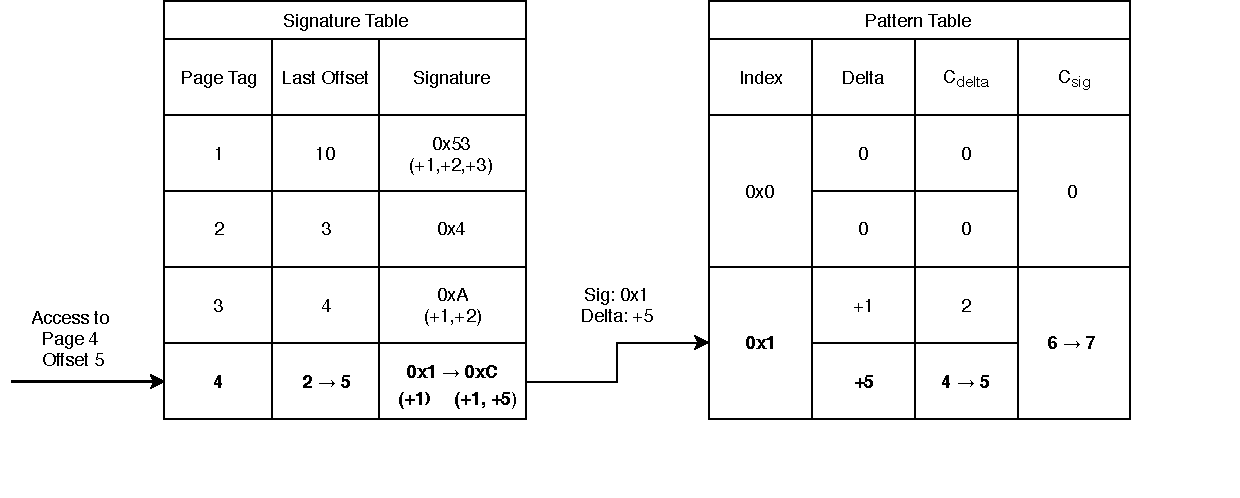
\includegraphics[width=\columnwidth]{SPP_Update_Description}
  \caption{SPP Data-path Flow}
  \label{fig:spp_update}
  \end{center}
\end{figure}


\begin{figure}
  \begin{center}
  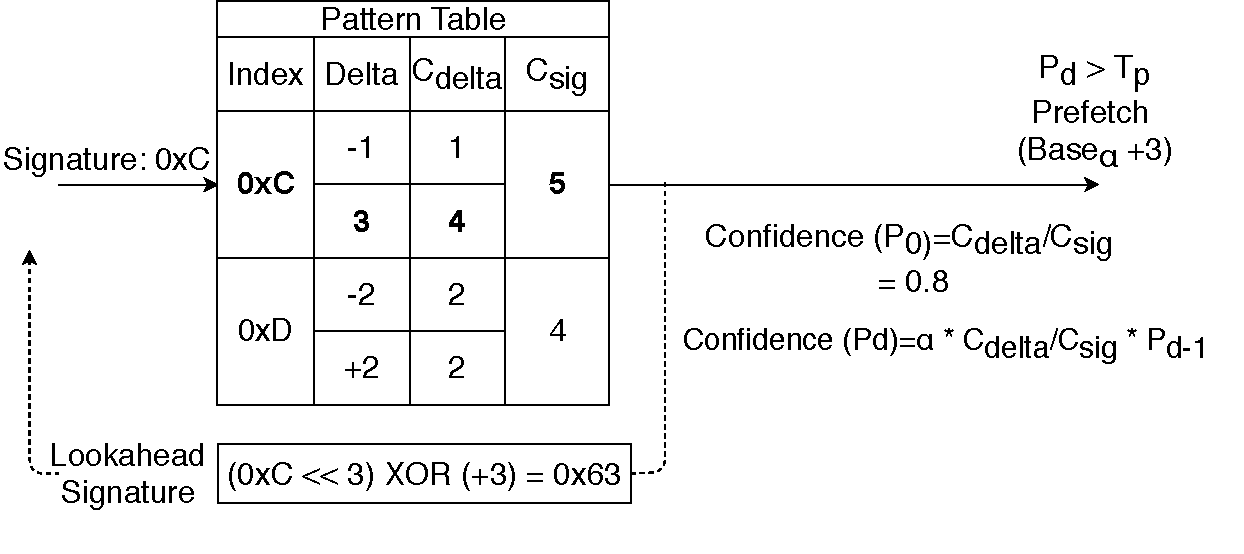
\includegraphics[width=\columnwidth]{SPP_Prefetch_Description}
  \caption{SPP Architecture}
  \label{fig:spp_structure}
  \end{center}
\end{figure}


% djimenez: this detail is unnecessary and likely to invite questions.
% reviewers might ask "what about linear separability?" but the proof is in the
% pudding.
%This form of indexing makes sure that the hyper-plane learned by the
%perceptron weights is able to differentiate between linearly
%inseparable outcomes. 

%\textit{Deviations From Actual Perceptrons:} Traditionally, a perceptron
%prediction involves multiplying the vector of input features:
%F\textsubscript{1xN}, with the corresponding weight vector:
%W\textsubscript{Nx1} in a dot product to obtain the sum y\textsubscript{out}.
%Here what we use is a perceptron-like structure.  The feature is used to hash
%into the weight of perceptrons and the retrieved weights are added straight
%away.  Thus, the perceptron algorithm doesn't introduce any multiplication
%operations in the inference or training process.  Hence what we adapt in this
%work is a perceptron-like learning algorithm as it involves the same principle
%involved in perceptron inferencing and training.

\subsection{Case for an On-line Filter}
\label{Background-Case}

%% Compared to some of the other state of the art prefetchers, SPP is
%% less aggressive.  In a single-core environment, there is no resource
%% contention among the different cores, hence aggressive prefetching is bound to prove beneficial. 
%% As we increase the core
%% count, we observe that SPP starts outperforming rest of the prefetchers.  This
%% can be attributed to the fact that each prefetch suggested by SPP is a
%% carefully calculated and prevents cache pollution.  \textit{<Figure
%% showing the variation of SPP vs BOP wrt core count>} For 4-core applications,
%% SPP suggests XX\% fewer prefetches than Best Offset Prefetcher ~\cite{bop} and yet leads to higher IPC.
%% 
%% The above analysis shows that with a more careful filtering mechanism, any
%% prefetcher like SPP can be tuned to become much more aggressive, yielding higher coverage.  The responsibility of maintaining high accuracy now falls on the
%% independent filter.  To test the hypothesis, we tuned down SPP to the
%% minimum possible threshold, with the effect of increasing prefetch suggestions
%% made by SPP by XX\%.  \textit{<Comparison of SPP-Unleased with SPP / BOP>}
%% Obviously this came at a cost of increased DRAM traffic and cache pollution.

% EB: This remains one of the untouched subsections of the paper

As was noted in Figure~\ref{Fig:Motivation}, an aggressive lookahead
prefetching, if done without any accuracy check, can harm the
performance of the system. As the figure shows, aggressive lookahead
and its accompanied loss of accuracy degrades performance by almost
9\%.  This is despite a growing number of useful prefetches generated
by the prefetcher.  Thus, we need a mechanism that is orthogonal to
the underlying prefetching scheme and can be used to prune out the
useful prefetches from the useless ones.

Moreover, the on-line confidence mechanism used by most prefetchers is
very rudimentary. For example, SPP's internal confidence mechanism is
based on taking the ratio C\textsubscript{d} = C\textsubscript{delta}
/ C\textsubscript{sig}. This confidence was used to make the decision
of whether to prefetch or not to prefetch; and which level to
prefetch.  While this approximation was shown to work in the original
implementation, we believe that a better form of generalized on-line
decision making was possible. Hence, it was necessary to build a
robust and adaptable learning mechanism to accept / reject the
prefetch suggestions; and to decide the fill level (L2 Cache vs Last
Level Cache). Thus, we introduce an independent on-line perceptron
based filtering mechanism.

\subsection{Perceptron Learning}
\label{sec:Background-Perceptron}
Perceptron learning for microarchitectural prediction was introduced
for branch prediction~\cite{PerceptronPredictor}. Our predictor uses a
version of microarchitectural perceptron prediction known as the
``hashed perceptron'' organization~\cite{HashedPerceptron}. As an
abstract idea, a hashed perceptron predictor hashes several different
features into values that index several distinct tables. Small integer
weights are read out from the tables and summed. If the sum exceeds
some threshold, a positive prediction is made, {\em e.g.} ``predict
branch taken'' or ``allow the prefetch.'' Otherwise, a negative
prediction is made. Once the ground truth is known, the weights
corredponding to the prediction are incremented if the outcome was
positive, or decremented if it was negative. This update only occurs
if the prediction was incorrect or if the magnitude of the sum failed
to exceed a threshold.  Beyond branch prediction, perceptron learning
has been applied to last-level cache reuse
prediction~\cite{Perc_Reuse,Multiperspective}. In this paper, we apply
it for the first time to prefetch filtering.

%\textit{Perceptron Learning Rule:} In a perceptron-based mechanism, a uniform
%perceptron update principle is followed.  The weights need to be updated if
%the prediction was wrong or the magnitude of the dot product does not exceed a
%certain threshold.  After a certain training period, these weights are
%proportional to the probability of a correct prediction.  Thresholding the
%outcome to a
% magnitude makes sure the perceptrons are trained until a certain level of
%confidence and yet they are not over-trained to the given set.  The perceptron
%learning rule will be applied to PPF.


%ETG: this is what I had added about perceptrons, we're trying to 
%figure out what to leave and what to get rid of ...  
% djimenez: I ended up cutting everything you wrote as well as the figure. I
% wrote something similar above, and the perceptron model described here isn't
% the hashed perceptron that we're using but rather the dot-product model from
% the original paper.

%\subsection{Perceptron-based Prediction}
%
%Perceptrons in microarchitecture were first introduced by Jimenez and Lin~\cite{PerceptronPredictor} 
%for branch prediction. In this work, a perceptron weights vector is selected by a hash of 
%the branch address and its dot product with an input vector of the previous branch history 
%outcomes. If the product is at least 0, the branch is predicted as taken, otherwise it is 
%predicted not taken. The weights are updated with the perceptron update rule: if the prediction 
%is incorrect, or the dot product does not exceed some threshold magnitude, then the weights 
%are incremented or decremented based on their correlation to the corresponding history bits. 
%Perceptron learning yields to superior accuracy, which results in increased opportunity for 
%optimizations.

%\begin{figure}[ht]
%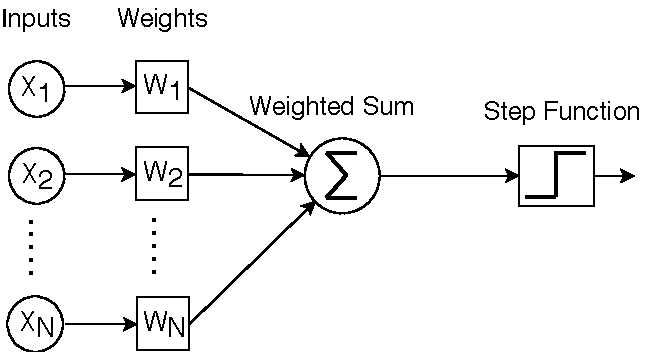
\includegraphics[width=\columnwidth]{Perc_Model}
%\caption{The Basic Perceptron Model}
%\label{Fig:Perc_Model}
%\end{figure}

%\subsubsection{Perceptron Learning}
%
%In a perceptron-based mechanism, a uniform perceptron update principle is
%followed. As shown in the figure~\ref{Fig:Perc_Model} Perceptrons are a simple
%model of neurons in neural networks \cite{perceptrons1,perceptrons2} modeled
%by vectors of signed weights learned through online training. The output of a
%perceptron is the dot product of the weights and a vector of inputs. In this
%work, we make use of the perceptron learning algorithm. There are two
%components to the abstract perceptron learning algorithm:
%
%\begin{enumerate}
%\item To predict true or false, a vector of signed weights is chosen according to some criteria. 
%The dot product of the weights and input vectors, called $y_{\mbox{\small out}}$, is computed. 
%If $y_{\mbox{\small out}}$ exceeds some threshold, the prediction is true, otherwise it is false.
%
%\item To update the weights after the true outcome of the predicted event is
%known, we first consider the value of $y_{\mbox{\small out}}$. If the
%prediction was correct and $|y_{\mbox{\small out}}|$ exceeds a threshold
%$\theta$, then the weights remain unchanged. Otherwise, the inputs are used to
%update the corresponding weights.  If there is positive correlation between
%the input and the outcome of the event, the corresponding weight is
%incremented; otherwise, it is decremented. Over time, the weights are
%proportional to the probability that the outcome of the event is true in the
%context of the input and the criterion for choosing that weight. The weights
%saturate at maximum and minimum values so they will fit in a fixed bit width.
%\end{enumerate}
